\section{Specification of Buddy Allocation Model}
The specification of the buddy memory management consists of a model for the necessary data structures to represent the memory, and for the allocation and disposal operations that memory management provides. This specification follows the algorithms for the buddy memory management in Zephyr OS, which applies a quartering split over blocks.

\subsection{State Representation}
\label{statedes}
The specification begins with the structure of a quad-tree.
{\footnotesize
\begin{align*}
&(set:\ 'a)\ tree\ =\ Leaf\ (L:\ 'a)\ | \\
&Node\ (LL:\ 'a\ tree)\ (LR:\ 'a\ tree)\ (RL:\ 'a\ tree)\ (RR:\ 'a\ tree)
\end{align*}
}
We use recursive method to construct a quad-tree. It has two forms: \emph{Leaf} tree and \emph{Node} tree. A \emph{Node} tree is built by itself or a \emph{Leaf} tree. The notation \emph{Leaf} means the end of this construct process. Notations \emph{LL}, \emph{LR}, \emph{RL} and \emph{RR} return corresponding subtrees of the \emph{Node} tree. Notation \textbf{set} means a function that gathers polymorphic notation \emph{'a} of all the leaves as a collection.
{\footnotesize
\begin{align*}
block\_state\_type\ &=\ FREE\ |\ ALLOC \\
ID\ &=\ nat \\
Block\ &=\ (block\_state\_type\ \times\ ID)\ tree
\end{align*}
}
In this specification, we use tuple type (\emph{block\_state\_type} $\times$ \emph{ID}) to instantiate the polymorphic notation \emph{'a} in the quad-tree structure. Type \emph{block\_state\_type} stands for the usage state of a block. It consists of two subtypes indicated as \emph{ALLOC} and \emph{FREE} constructed by \emph{datatype} function. Another type \emph{ID} in basic type \emph{nat} represents a range of address occupied by a memory block. Finally, type \emph{Block} represents an instantiated quad-tree.

In addition, we create some auxiliary functions to manipulate the \textsl{block tree}. Function \textbf{get\_level} takes two Blocks \emph{btree} and \emph{b} as inputs, then returns a nat \emph{level} which represents the layer number that \emph{b} locates in \emph{btree} from the root whose layer number is 0. Function \textbf{allocsets} takes a Block \emph{btree} and returns a Block set \emph{aset} of all Leaf nodes whose \emph{block\_state\_type} is \emph{ALLOC} from \emph{btree}. Function \textbf{freesets} has a similar definition but returns \emph{FREE} ones. Function \textbf{freesets\_level} takes a Block \emph{btree} and a nat \emph{level}, then returns a Block set \emph{fset} of all Leaf nodes whose \emph{block\_state\_type} is \emph{FREE} and locate at \emph{level} in \emph{btree}. We use a notation \emph{idset} to represent the collection of all used \emph{IDs}. To create a new Leaf node, we have to pick up a new \emph{ID} to mark it by the strategy of \emph{SOME p. p} $\notin$ \emph{idset}.

Before introducing allocation model, we create a function \textbf{output\_level} that maps request sizes to the most suitable allocation levels in a quad-tree. The input parameters are a nat list \emph{blo\_list} and a nat \emph{rsize}. Static linked list \emph{blo\_list} is used to store the size of blocks for each level in a quad-tree and its indexes represent the levels of a quad-tree. For example, the size of root is 1024\emph{Mbytes} and the first level is 256\emph{Mbytes}, then \emph{blo\_list}!0 is equal to 1024 and \emph{blo\_list}!1 is 256. The \emph{blo\_list} is a strictly decreasing list to simulate the fact that the smaller the level, the larger size the memory block. The function returns a nat index \emph{l} in \emph{blo\_list} with these constrains: the size it represents has to be greater than or equal to the size of request block, and there is no smaller size that meets this condition. After that, the most suitable block size is picked up from \emph{blo\_list}, and then mapped to the correct level of the quad-tree by the index \emph{l} in \emph{blo\_list}. We use \emph{rlv} to represent the output. The definition of this mapping is as follows.

\begin{definition} [Mapping Request Sizes to Allocation Levels]
\label{mostsuitable}
\end{definition}
\vspace{-7pt}
{\footnotesize
\begin{align*}
&output\_level\ blo\_list\ rsize \triangleq THE\ l.\ l < \vert blo\_list \vert \\
&\wedge rsize \le blo\_list\ !\ l \\
&\wedge ((\vert blo\_list \vert > 1 \wedge l < \vert blo\_list \vert - 1) \longrightarrow rsize > blo\_list\ !\ (l+1))
\end{align*}
}
\vspace{-17pt}

\subsection{Allocation Model}
Now we specify allocation operation as function \textbf{alloc}. Firstly, we introduce two assistant functions. Function \textbf{exists\_freelevel} takes a Block set \emph{bset} and a nat \emph{rlv} as inputs, then returns a bool result \emph{re} represents whether there is a Block in \emph{bset} (the collection of all quad-trees in memory system) that has such \emph{FREE} Leaf nodes whose level is less than or equal to \emph{rlv}. Function \textbf{freesets\_maxlevel} has the same inputs, but returns a nat \emph{lmax} represents the maximum level among all levels with \emph{FREE} Leaf nodes but less than or equal to \emph{rlv}. The definitions are as follows.

\begin{definition} [existence of free blocks in a level]
\end{definition}
\vspace{-7pt}
{\footnotesize
\begin{align*}
exists\_freelevel\ bset\ rlv &\triangleq \exists l.\ l \leq rlv \\
&\wedge \exists b \in bset.\ freesets\_level\ b\ l \ne \emptyset
\end{align*}
}
\vspace{-12pt}

\begin{definition} [maximum level of free blocks]
\end{definition}
\vspace{-7pt}	
{\footnotesize
\begin{align*}
&freesets\_maxlevel\ bset\ rlv \triangleq THE\ lmax.\ lmax \leq rlv \\
&\wedge \exists b \in bset.\ freesets\_level\ b\ lmax \neq \emptyset \\
&\wedge (\forall l \leq rlv.\ \exists b \in bset.\ freesets\_level\ b\ l \ne \emptyset \longrightarrow l \leq lmax)
\end{align*}
}
\vspace{-12pt}

During the allocation process, if no such Leaf node right in the requested level exists but bigger Leaf nodes exist, then it is necessary to split a bigger Leaf node into small Leaf nodes until a Leaf node that satisfies the request appears. Function \textbf{split} divides a Leaf node \emph{b} into a Node \emph{btree} by recursion for a nat \emph{lv} times. It invokes a function \textbf{divide} that takes a Leaf node \emph{b} and returns a new non-terminal Node \emph{n} with four terminal Leaf nodes. The leftmost Leaf of \emph{n} is marked as \emph{ALLOC}, while the rests are marked as \emph{FREE}. The division operation always conducts on the leftmost subtree. A simple example describing this process is showed in Fig. \ref{fig1} until \emph{FREE} Leaf in the request level appears and then be allocated. We define the \emph{split} operation as follows.

\begin{figure}[htbp]
	\centering
	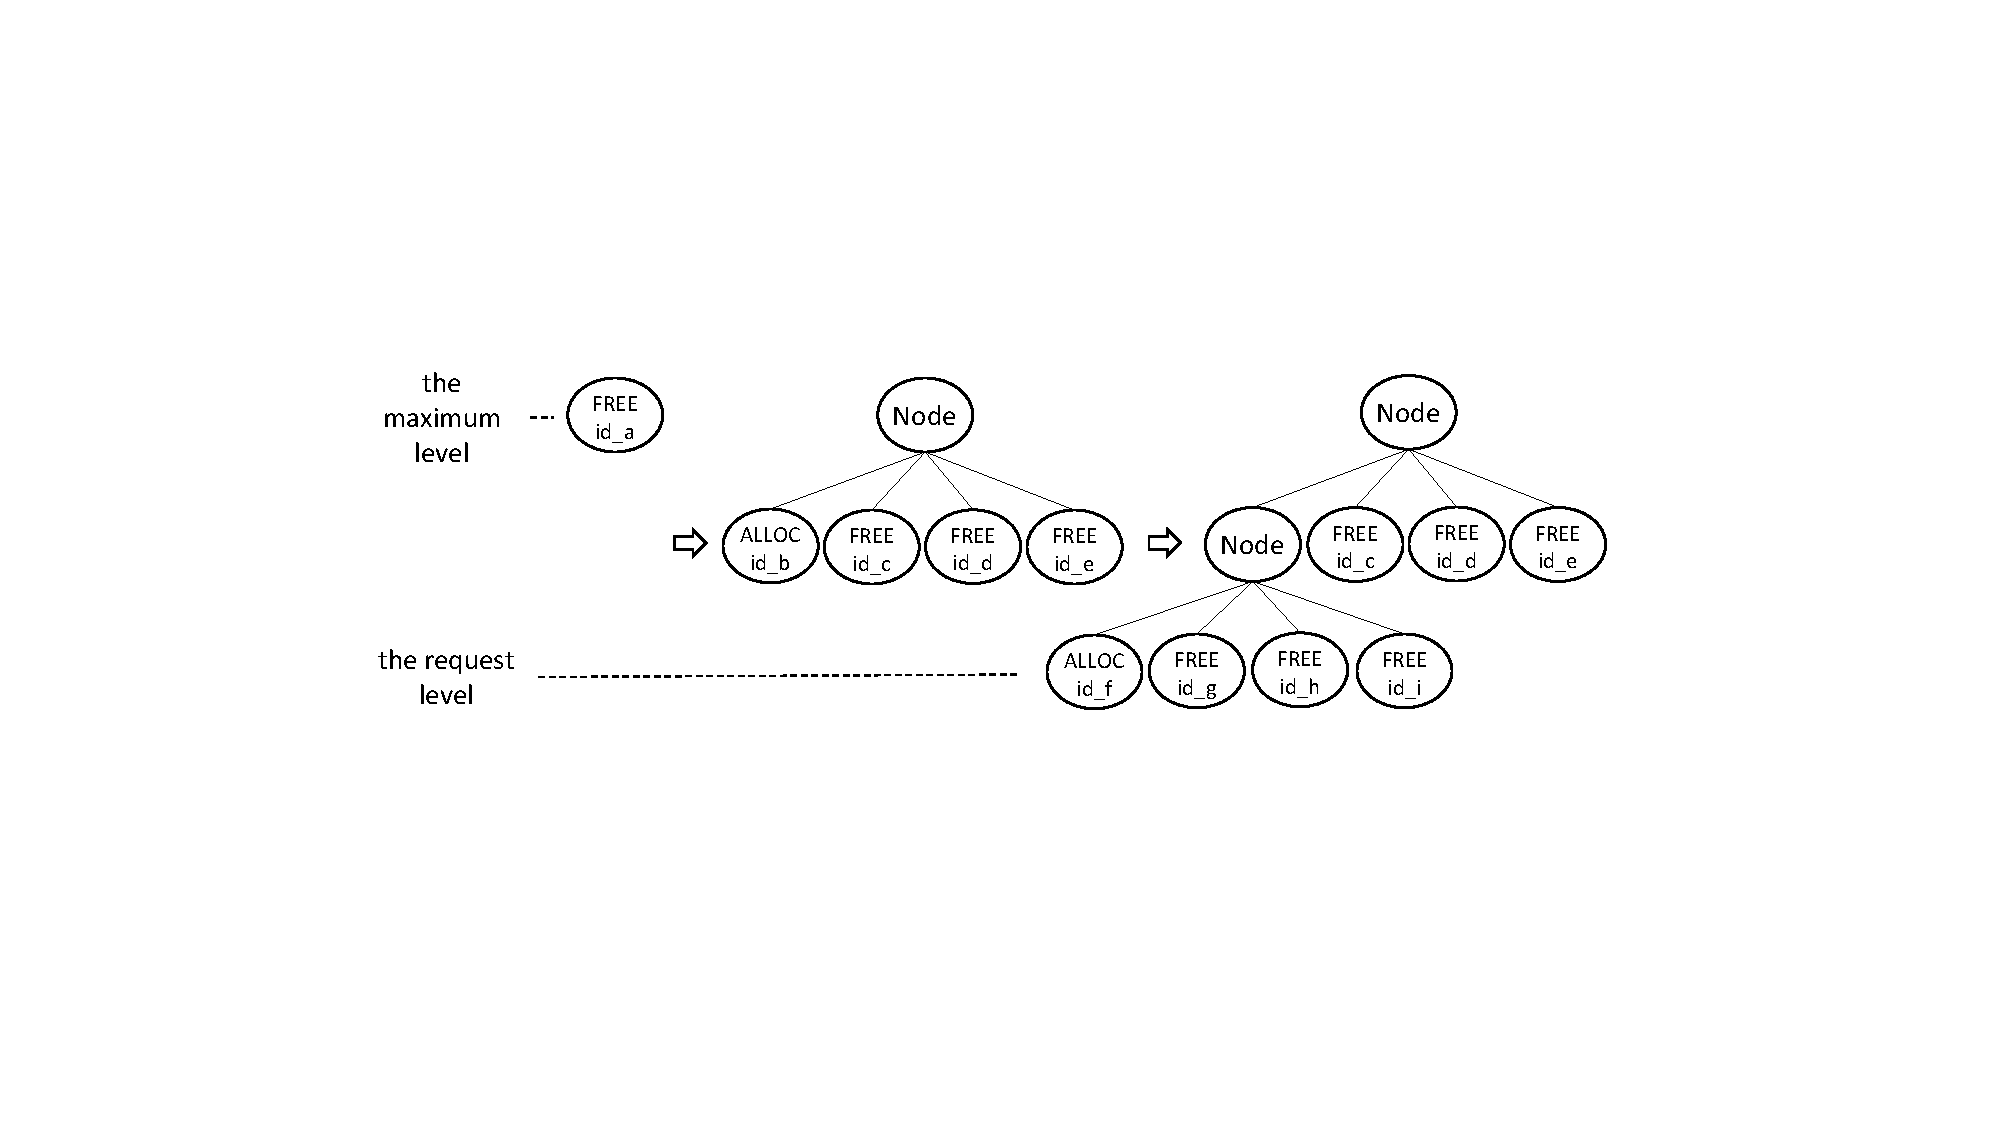
\includegraphics[width=0.5\textwidth]{fig1.pdf}
	\caption{The progress of dividing a free leaf}
	\label{fig1}
\end{figure}

\begin{definition} [splitting a leaf]
\end{definition}
\vspace{-7pt}
{\footnotesize
\begin{align*}
split\ b\ lv \triangleq\ &if\ lv = 0\ then\ b \\
else\ Node\ &(split\ (LL\ divide\ b)\ (lv - 1))\ (LR\ divide\ b)\\ 
&(RL\ divide\ b)\ (RR\ divide\ b)
\end{align*}
}	
\vspace{-12pt}

In addition, we give functions \textbf{set\_type}, \textbf{replace} and \textbf{replace\_leaf} as follows: function \emph{set\_type} takes a Leaf node \emph{b} and a target block\_state\_type \emph{s}, then changes the type of \emph{b} with \emph{s}, finally returns it as a new Leaf node \emph{b'}. function \emph{replace} takes a Block \emph{btree}, two Leaf nodes \emph{b} and \emph{b'} as inputs, then replace the Leaf node \emph{b} with \emph{b'} in \emph{btree}, finally returns the updated Block \emph{btree'}. function \emph{replace\_leaf} takes a Block \emph{btree}, a Leaf node \emph{b} and a Node \emph{btr} as inputs, then replace the Leaf node \emph{b} with \emph{btr} in \emph{btree}, lastly returns the updated Block \emph{btree'}. 

Now we give the process of allocation operation. It firstly checks whether there is Block in \emph{bset} that has such \emph{FREE} Leaf nodes whose level is less than or equal to \emph{rlv} by function \emph{exists\_freelevel}. If it returns \emph{False} then the allocation process stops and returns original \emph{bset} and \emph{False}. Otherwise, function \emph{freesets\_maxlevel} returns the maximum level \emph{lmax} among all levels with \emph{FREE} Leaf nodes but less than or equal to \emph{rlv}. Two branches are as follows.

If the \emph{lmax} is equal to requested level \emph{rlv} then: randomly pick up such a Block as \emph{btree}; pick up such a \emph{FREE} Leaf node \emph{l} in level \emph{rlv} from \emph{btree}; invoke \emph{set\_type} to set \emph{l} type \emph{ALLOC} as \emph{l'}; invoke \emph{replace} to update \emph{btree} with \emph{l'} as \emph{btree'}; finally return updated Block set \emph{bset} with \emph{btree'} and \emph{True}.

If the \emph{lamx} is not equal to requested level \emph{rlv} then: randomly pick up such a Block as \emph{btree} who has \emph{FREE} Leaf nodes in level \emph{lmax}; pick up such a \emph{FREE} Leaf node \emph{l} in level \emph{lmax} from \emph{btree}; invoke \emph{split} to split \emph{l} into Node \emph{btr}; invoke \emph{replace\_leaf} to update \emph{btree} with \emph{btr} as \emph{btree'}; finally return updated Block set \emph{bset} with \emph{btree'} and \emph{True}. The definition of allocation operation is as follows.

\begin{definition} [Allocation Operation]
\end{definition}
\vspace{-7pt}
{\footnotesize
\begin{align*}
alloc\ &bset\ rlv \triangleq \\
&if\ exists\_freelevel\ bset\ rlv\ then \\
&\ \ \ \ lmax = freesets\_maxlevel\ bset\ rlv \\
&\ \ \ \ if\ lmax = rlv\ then \\
&\ \ \ \ \ \ \ \ btree = SOME\ b.\ b \in bset \wedge freesets\_level\ b\ rlv \ne \emptyset \\
&\ \ \ \ \ \ \ \ l = SOME\ l.\ l \in freesets\_level\ btree\ rlv \\
&\ \ \ \ \ \ \ \ btree' = replace\ btree\ l\ (set\_type\ l\ ALLOC) \\
&\ \ \ \ \ \ \ \ return\ (bset - \lbrace btree \rbrace \cup \lbrace btree' \rbrace, True) \\
&\ \ \ \ else \\
&\ \ \ \ \ \ \ \ btree = SOME\ b.\ b \in bset \wedge freesets\_level\ b\ lmax \ne \emptyset \\
&\ \ \ \ \ \ \ \ l = SOME\ l.\ l \in freesets\_level\ btree\ lmax \\
&\ \ \ \ \ \ \ \ btr' = split\ l\ (rlv - lmax) \\
&\ \ \ \ \ \ \ \ btree' = replace\_leaf\ btree\ l\ btr' \\
&\ \ \ \ \ \ \ \ return\ (bset - \lbrace btree \rbrace \cup \lbrace btree' \rbrace, True) \\
&else\ return\ (bset, False)
\end{align*}
}
\vspace{-17pt}

\subsection{Deallocation Model}
During the deallocation process, if such a situation that four Leaf nodes belonging to a same parent Node are all \emph{FREE} appears, function \textbf{merge} is invoked to merge these Leaf nodes to one Leaf node. It invokes a function \textbf{combine} that takes a Node \emph{n} and returns a new terminal Leaf node \emph{l} \emph{iff} Node \emph{n} has four terminal \emph{FREE} Leaf nodes. Function \emph{merge} takes a Node \emph{n} and recursively invokes \emph{combine} on each sub-node of \emph{n} and \emph{n} itself. A simple example that describes the merging process is showed in Fig. \ref{fig2}.

\begin{figure}[htbp]
	\centering
	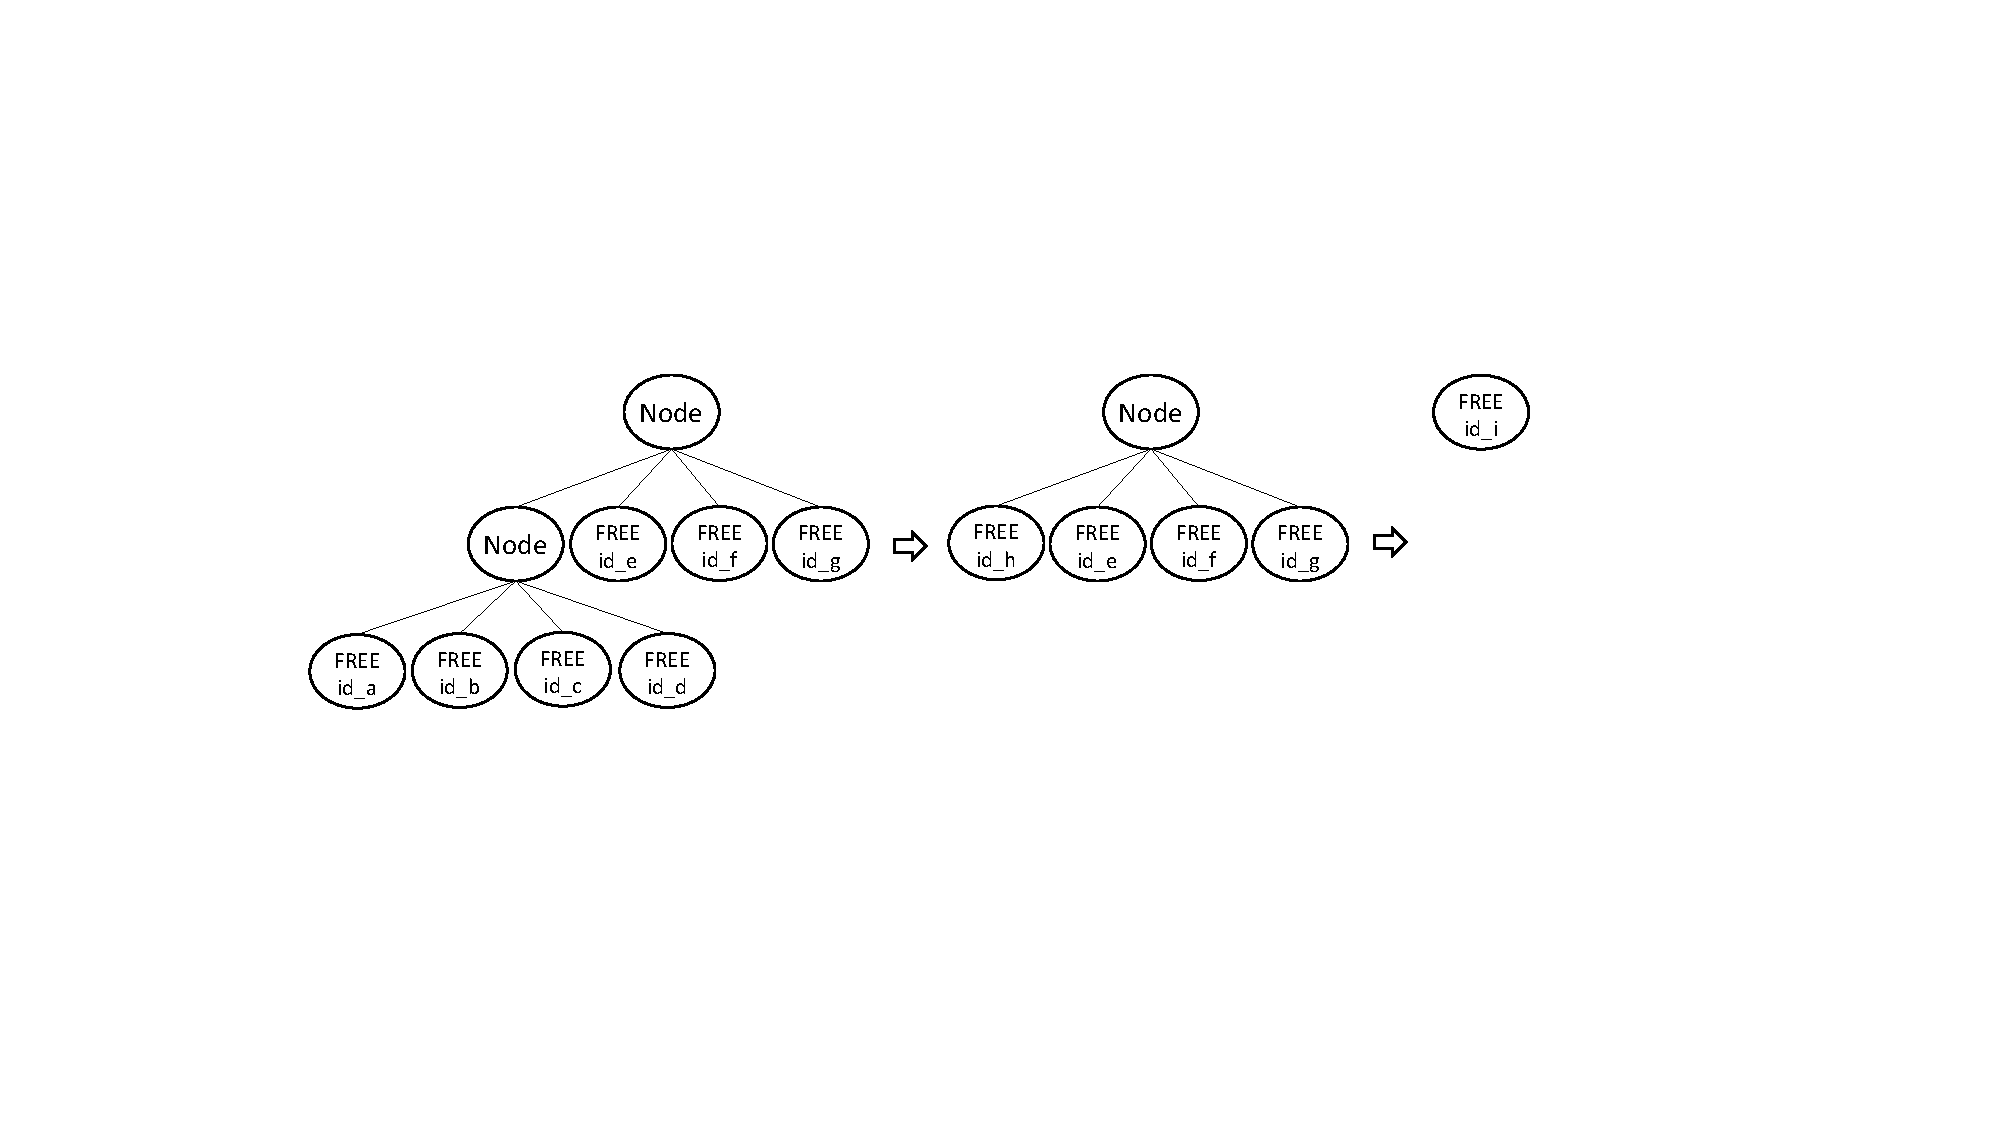
\includegraphics[width=0.5\textwidth]{fig2.pdf}
	\caption{The progress of merging all free memory blocks}
	\label{fig2}
\end{figure}

With above discussion, we give the process of deallocation operation. It firstly checks whether there is a Block in \emph{bset} that the Leaf node \emph{b} to be deposed belongs to it. If there is no such tree, the procedure returns the original \emph{bset} and \emph{False}. Otherwise, if the type of \emph{b} is \emph{FREE}, it also returns the original \emph{bset} and \emph{False}. When all conditions are met, it picks up the Block in \emph{bset} that \emph{b} belongs to as \emph{btree}; invokes \emph{set\_type} to set \emph{b} type \emph{FREE} as \emph{b'}; invokes \emph{replace} to update \emph{btree} with \emph{b'} as \emph{btree'}; invokes \emph{merge} to perform a necessary merging operation on \emph{btree'} as \emph{btree''}; finally returns updated Block set \emph{bset} with \emph{btree''} and \emph{True}. The definition of deallocation operation is as follows.

\begin{definition} [Deallocation Operation]
\end{definition}
\vspace{-7pt}
{\footnotesize
\begin{align*}
free\ &bset\ b \triangleq \\
&if\ \exists btree \in bset.\ b \in set\ btree\ then \\
&\ \ \ \ if\ fst\ b = FREE\ then \\
&\ \ \ \ \ \ \ \ return\ (bset, False) \\
&\ \ \ \ else \\
&\ \ \ \ \ \ \ \ btree = THE\ t.\ t \in bset \wedge b \in set\ t \\
&\ \ \ \ \ \ \ \ btree' = replace\ btree\ b\ (set\_type\ b\ FREE) \\
&\ \ \ \ \ \ \ \ btree'' = merge\ btree' \\
&\ \ \ \ \ \ \ \ return\ (bset - \lbrace btree \rbrace \cup \lbrace btree'' \rbrace, True) \\
&else\ return\ (bset, False)
\end{align*}
}
\vspace{-12pt}

At this point, we have done the specification for the buddy memory algorithms. Next, we are going to verify its functional correctness and security property.